\chapter{Implementação}
\label{c.implementacao}
A implementação foi feita através de um script em Matlab elaborado pelo autor. O script recebe como \emph{input} os dados históricos de todos os dias de um intervalo de anos para uma cidade, e então gera os resultados como \emph{\emph{output}}. A base de dados, inputs, outputs e o script serão tratados com detalhes nos tópicos a seguir.

\section{Base de Dados}
\label{s.basedados}
Para a base de dados, a cidade escolhida foi Bauru, no estado de São Paulo. Bauru tem maiores quantidades de chuva durante o verão, com um inverno mais seco.

Todos os dados obtidos estão disponíveis livre e gratuitamente para consulta no site do Instituto Nacional de Meteorologia (INMET) ~\cite{inmet}. A estacão que mediu os dados tem o código de A705, com local em latitude -22,358052, longitude -49,028877 e altitude de 636,17m. Os dados foram medidos dia a dia, durante todos os meses dos anos de 2002 a 2020, sendo no total 19 anos (6935 dias) de dados. Os dias 29 de fevereiro de cada ano foram desconsiderados por não ter uma quantidade suficiente de dados. 

Os dados disponibilizados são horários, diários ou mensais, de estacões convencionais ou automáticas. Além de dados sobre precipitação, também podem ser consultados dados de temperatura, umidade, vento e pressão atmosférica. As unidades dos dados são:
\begin{itemize}
    \item Temperatura média, máxima, mínima e do ponto de orvalho média (\degree C);
    \item Umidade Relativa do Ar média e mínima (\%);
    \item Precipitação Total (mm);
    \item Velocidade média e rajada máxima do Vento (km/h, m/s);
    \item Pressão atmosférica média (atm).
\end{itemize}


%é

\section{Inputs e Outputs}
\label{s.io}
Para que o script possa funcionar, ele precisa de alguns dados de entrada, chamados de \emph{inputs}. Através desses dados é realizado todo o processamento para então gerar os dados de saída, chamados de \emph{outputs}.
Esses dados devem estar em formatos específicos para atender as necessidades do programa. Caso contrario, o script não funcionará corretamente e acabará em erros.

\subsection{Inputs}
\label{ss.inputs}
Para os dados de entrada, chamados de \emph{inputs}, o script precisa de 12 arquivos em formato .txt que funcionam como matrizes, cada um representando cada mês, de janeiro a dezembro. Cada um desses arquivos deve ter 31 linhas, representando os dias, e no mínimo 2 colunas, representando a base histórica dos anos. Além desses 12 arquivos, um arquivo extra é necessário com a precipitação diária do dia anterior ao dia mais antigo da base de dados, pois a Cadeia de Markov a qual o modelo se baseia utiliza dados dos dias anteriores para gerar as probabilidades condicionais necessárias. Dentro desses arquivos devem estar dados da precipitação diária em milímetros, separados por espaços e com casas decimais delimitadas por um ponto em vez de vírgula, provenientes diretamente da base de dados escolhida. 

O quadro \ref{q.input} demonstra um exemplo de um arquivo .txt que pode ser utilizado como \emph{input}. Percebe-se que o quadro tem 31 linhas, que representam os dias, e 3 colunas, que representam uma base histórica de três anos para um determinado mês. Assim, se a coluna 2 representar o ano de 2019, a terceira linha será o dia 3 de janeiro, portanto o script tem a informação de que a precipitação diária do dia 3 de janeiro de 2019 foi 1,4mm.

Para dados reais, quanto maior o número de colunas, melhor será a simulação pluviométrica. Isso acontece porque as colunas representam os anos, e a Cadeia de Markov tem um grau de precisão maior conforme o número de dados históricos é aumentado.

\begin{table}[H]
\caption{Exemplo de \emph{input} utilizado pelo script para o processamento da simulação.}
\label{q.input}
\centering

\begin{tabular}{|c|c|c|}
\hline
0.2 & 0   & 0.4  \\ \hline
0   & 0   & 0    \\ \hline
17  & 1.4 & 0    \\ \hline
0   & 0   & 2    \\ \hline
0   & 6.8 & 2    \\ \hline
0   & 0   & 0    \\ \hline
0   & 0   & 0    \\ \hline
0   & 9   & 0    \\ \hline
5   & 12  & 16.8 \\ \hline
0   & 10  & 0    \\ \hline
0   & 0   & 0    \\ \hline
0   & 0   & 0    \\ \hline
6   & 0   & 0    \\ \hline
0.8 & 0   & 0    \\ \hline
2   & 0   & 0    \\ \hline
0   & 0   & 0    \\ \hline
0   & 0   & 0    \\ \hline
0   & 9   & 0    \\ \hline
0   & 4   & 0    \\ \hline
0   & 0   & 34   \\ \hline
1.6 & 0   & 0    \\ \hline
0   & 0   & 0    \\ \hline
0   & 0   & 5    \\ \hline
0   & 0   & 0    \\ \hline
0   & 6   & 0    \\ \hline
0   & 0   & 4    \\ \hline
9   & 0   & 16   \\ \hline
0   & 0   & 0    \\ \hline
0   & 5   & 0    \\ \hline
0   & 0   & 0    \\ \hline
3.8 & 0   & 23   \\ \hline
\end{tabular}
\vspace*{15px}
\legend{\small Fonte: Elaborado pelo autor.}
\end{table}

\subsection{Outputs}
\label{ss.outputs}
Depois de processados os dados de entrada, o script gera automaticamente, em milésimos de segundos, o resultado bruto da simulação com base no modelo estudado.

São dois os resultados gerados, também em formato .txt representando matrizes. O primeiro deles é uma matriz com 31 linhas e 12 colunas, ou seja, um ano inteiro simulado, com probabilidades de chuva entre 0 e 1 separadas por um espaço simples, conforme demonstrado no quadro \ref{q.output1}. O segundo output, e o mais importante, também é uma matriz com 31 linhas e 12 colunas, mas com dados binários (0 ou 1) representando se os dias vão ser secos ou chuvosos, respectivamente. O quadro \ref{q.output2} demonstra um exemplo do segundo resultado gerado pelo script.

\begin{table}[H]
\caption{Exemplo de output com probabilidades condicionais gerado pelo script.}
\label{q.output1}
\centering
\begin{tabular}{|c|c|c|c|c|c|c|c|c|c|c|c|}
\hline
0,26 & 0,61 & 0,90 & 0,02 & 0,33 & 0,23 & 0,63 & 0,03 & 0,50 & 0,25 & 0,49 & 0,23 \\ \hline
0,65 & 0,23 & 0,07 & 0,63 & 0,57 & 0,30 & 0,88 & 0,73 & 0,89 & 0,61 & 0,30 & 0,06 \\ \hline
0,35 & 0,09 & 0,32 & 0,92 & 0,11 & 0,82 & 0,10 & 0,88 & 0,84 & 0,56 & 0,67 & 0,84 \\ \hline
0,65 & 0,77 & 0,02 & 0,90 & 0,84 & 0,52 & 0,56 & 0,07 & 0,26 & 0,03 & 0,87 & 0,59 \\ \hline
0,66 & 0,55 & 0,35 & 0,56 & 0,76 & 0,65 & 0,67 & 0,64 & 0,06 & 0,31 & 0,92 & 0,99 \\ \hline
0,53 & 0,73 & 0,83 & 0,60 & 0,03 & 0,89 & 0,76 & 0,15 & 0,99 & 0,20 & 0,40 & 0,34 \\ \hline
0,74 & 0,20 & 0,84 & 0,99 & 0,95 & 0,56 & 0,40 & 1,00 & 0,73 & 0,99 & 0,96 & 0,12 \\ \hline
0,14 & 0,83 & 0,46 & 0,95 & 0,44 & 0,86 & 0,66 & 0,76 & 0,63 & 0,98 & 0,00 & 0,51 \\ \hline
0,61 & 0,48 & 0,35 & 0,76 & 0,09 & 0,44 & 0,10 & 0,34 & 0,28 & 0,61 & 0,19 & 0,24 \\ \hline
0,22 & 0,76 & 0,87 & 0,29 & 0,97 & 0,06 & 0,26 & 0,32 & 0,24 & 0,85 & 0,14 & 0,54 \\ \hline
0,87 & 0,96 & 0,36 & 0,79 & 0,22 & 0,99 & 0,25 & 0,68 & 0,84 & 0,17 & 0,85 & 0,48 \\ \hline
0,30 & 0,05 & 0,36 & 0,11 & 0,20 & 0,73 & 0,61 & 0,80 & 0,56 & 0,67 & 0,83 & 0,46 \\ \hline
0,18 & 0,74 & 0,28 & 0,35 & 0,06 & 0,25 & 0,16 & 0,72 & 0,98 & 0,91 & 0,88 & 0,77 \\ \hline
0,01 & 0,70 & 0,73 & 0,63 & 0,22 & 0,08 & 0,97 & 0,53 & 0,62 & 0,79 & 0,96 & 0,10 \\ \hline
0,35 & 0,50 & 0,28 & 0,69 & 0,72 & 0,43 & 0,71 & 0,46 & 0,79 & 0,71 & 0,92 & 0,66 \\ \hline
0,92 & 0,92 & 0,92 & 0,25 & 0,27 & 0,59 & 0,64 & 0,11 & 0,22 & 0,23 & 0,34 & 0,76 \\ \hline
0,36 & 0,54 & 0,36 & 0,39 & 0,68 & 0,69 & 0,81 & 0,04 & 0,49 & 0,70 & 0,22 & 1,00 \\ \hline
0,63 & 0,82 & 0,03 & 0,20 & 0,83 & 0,74 & 0,15 & 0,83 & 0,85 & 0,49 & 0,17 & 0,16 \\ \hline
0,10 & 0,21 & 0,06 & 0,99 & 0,46 & 0,91 & 0,48 & 0,65 & 0,60 & 0,13 & 0,06 & 0,84 \\ \hline
0,42 & 1,00 & 0,74 & 0,42 & 0,78 & 0,96 & 0,27 & 0,72 & 0,94 & 0,44 & 0,84 & 0,48 \\ \hline
0,22 & 0,32 & 0,48 & 0,86 & 0,12 & 0,51 & 0,78 & 0,97 & 0,25 & 0,76 & 0,16 & 0,11 \\ \hline
0,34 & 0,89 & 0,06 & 0,70 & 0,52 & 0,62 & 0,11 & 0,11 & 0,15 & 0,31 & 0,41 & 0,40 \\ \hline
0,44 & 0,96 & 0,66 & 0,18 & 0,90 & 0,12 & 0,23 & 0,82 & 0,21 & 0,05 & 0,23 & 0,40 \\ \hline
0,71 & 0,16 & 0,62 & 0,02 & 0,95 & 0,07 & 0,87 & 0,97 & 0,73 & 0,72 & 0,16 & 0,38 \\ \hline
0,86 & 0,89 & 0,49 & 0,85 & 0,00 & 0,90 & 0,93 & 0,32 & 0,62 & 0,80 & 0,11 & 0,66 \\ \hline
0,01 & 0,51 & 0,59 & 0,84 & 0,75 & 0,37 & 0,67 & 0,99 & 0,34 & 0,14 & 0,95 & 0,56 \\ \hline
0,34 & 0,35 & 0,40 & 0,29 & 0,53 & 0,22 & 0,17 & 0,04 & 0,10 & 0,13 & 0,20 & 0,46 \\ \hline
0,62 & 0,62 & 0,69 & 0,02 & 0,15 & 0,87 & 0,54 & 0,49 & 0,28 & 0,08 & 0,61 & 0,06 \\ \hline
0,69 & -    & 0,93 & 0,84 & 0,08 & 0,19 & 0,45 & 0,01 & 0,43 & 0,62 & 0,61 & 0,02 \\ \hline
0,24 & -    & 0,50 & 0,09 & 0,76 & 0,59 & 0,77 & 0,80 & 0,09 & 0,40 & 0,16 & 0,46 \\ \hline
0,47 & -    & 0,72 & -    & 0,51 & -    & 0,33 & 0,30 & -    & 0,60 & -    & 0,91 \\ \hline
\end{tabular}
\vspace*{15px}
\legend{\small Fonte: Elaborado pelo autor.}
\end{table}

\begin{table}[H]
\caption{Exemplo de output com dados binários gerado pelo script.}
\label{q.output2}
\centering
\begin{tabular}{|c|c|c|c|c|c|c|c|c|c|c|c|}
\hline
1 & 1 & 0 & 1 & 1 & 0 & 0 & 1 & 0 & 1 & 0 & 0 \\ \hline
0 & 1 & 1 & 1 & 0 & 1 & 1 & 0 & 1 & 1 & 0 & 0 \\ \hline
0 & 1 & 1 & 1 & 1 & 1 & 0 & 1 & 0 & 1 & 1 & 0 \\ \hline
0 & 1 & 1 & 1 & 1 & 1 & 1 & 1 & 1 & 1 & 1 & 1 \\ \hline
0 & 1 & 1 & 0 & 0 & 1 & 0 & 1 & 1 & 1 & 1 & 1 \\ \hline
0 & 1 & 0 & 1 & 0 & 0 & 0 & 1 & 0 & 1 & 1 & 1 \\ \hline
1 & 1 & 1 & 1 & 0 & 1 & 1 & 1 & 0 & 0 & 1 & 0 \\ \hline
1 & 0 & 1 & 1 & 1 & 1 & 0 & 0 & 1 & 0 & 1 & 0 \\ \hline
1 & 0 & 1 & 0 & 1 & 1 & 1 & 1 & 0 & 0 & 0 & 1 \\ \hline
0 & 1 & 0 & 1 & 0 & 0 & 1 & 1 & 0 & 0 & 1 & 0 \\ \hline
0 & 0 & 0 & 0 & 1 & 0 & 1 & 1 & 1 & 0 & 0 & 1 \\ \hline
1 & 1 & 0 & 0 & 1 & 0 & 0 & 0 & 1 & 1 & 1 & 0 \\ \hline
1 & 0 & 0 & 1 & 1 & 0 & 1 & 1 & 1 & 0 & 0 & 1 \\ \hline
0 & 0 & 1 & 0 & 0 & 1 & 1 & 1 & 1 & 0 & 0 & 0 \\ \hline
0 & 1 & 0 & 0 & 1 & 1 & 0 & 0 & 0 & 1 & 1 & 1 \\ \hline
0 & 1 & 0 & 0 & 0 & 1 & 0 & 1 & 1 & 1 & 1 & 0 \\ \hline
0 & 1 & 0 & 0 & 0 & 0 & 0 & 1 & 0 & 0 & 0 & 0 \\ \hline
1 & 1 & 0 & 1 & 1 & 1 & 1 & 0 & 0 & 0 & 0 & 0 \\ \hline
0 & 0 & 1 & 0 & 0 & 1 & 0 & 1 & 0 & 0 & 1 & 1 \\ \hline
1 & 0 & 1 & 0 & 0 & 1 & 1 & 0 & 1 & 1 & 1 & 1 \\ \hline
0 & 0 & 1 & 1 & 1 & 1 & 1 & 0 & 0 & 0 & 1 & 1 \\ \hline
1 & 0 & 1 & 0 & 1 & 0 & 0 & 1 & 0 & 0 & 1 & 1 \\ \hline
1 & 0 & 0 & 1 & 1 & 1 & 1 & 1 & 0 & 0 & 0 & 1 \\ \hline
0 & 0 & 1 & 1 & 0 & 1 & 0 & 1 & 1 & 1 & 0 & 1 \\ \hline
0 & 0 & 1 & 0 & 0 & 0 & 1 & 1 & 1 & 0 & 1 & 1 \\ \hline
0 & 1 & 1 & 0 & 1 & 0 & 0 & 1 & 1 & 1 & 1 & 0 \\ \hline
0 & 1 & 1 & 1 & 0 & 1 & 1 & 0 & 0 & 0 & 0 & 1 \\ \hline
1 & 1 & 1 & 1 & 0 & 0 & 1 & 1 & 1 & 0 & 0 & 0 \\ \hline
0 & - & 1 & 0 & 0 & 1 & 0 & 0 & 1 & 1 & 0 & 1 \\ \hline
0 & - & 1 & 1 & 1 & 1 & 1 & 0 & 0 & 0 & 1 & 1 \\ \hline
1 & - & 0 & - & 1 & - & 1 & 0 & - & 1 & - & 0 \\ \hline
\end{tabular}
\vspace*{15px}
\legend{\small Fonte: Elaborado pelo autor.}
\end{table}



\section{Script}
\label{s.io}
O script foi programado no ambiente de desenvolvimento do Matlab, então tem o formato .m padrão da linguagem. São 251 linhas de código comentadas e elaboradas de maneira eficiente para que o tempo de processamento seja o mais rápido possível.

O autor deixou disponível de maneira integral e aberta o script, bem como a base de dados e os resultados brutos da simulação em sua página do GitHub \cite{script-tcc} para que quaisquer interessados possam consultar ou até mesmo utilizar para algum projeto pessoal. Na figura \ref{f.example-script} é possível observar parte de uma função do script.

\begin{figure}[H]
	\caption{\small Parte de uma função do script.}
	\centering
	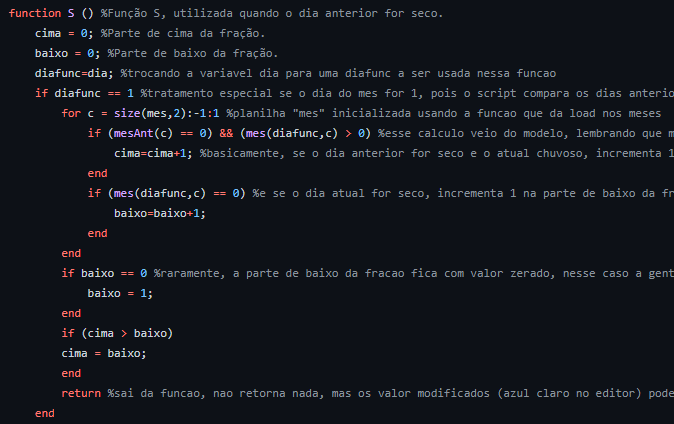
\includegraphics[width=\textwidth]{figs/example-script.png}
	\label{f.example-script}
	\legend{\small Fonte: Elaborado pelo Autor.}
\end{figure}







%é